%!TeX root = Thesis_LP.tex
\chapter{La géostatistique comme outil d’optimisation}
\label{sc:geostat}
Cette section résume brièvement les aspects théoriques et les démarches
méthodologiques effectuées pour répondre à l'objectif formulé dans la
\cref{sc:obj2}. La \cref{sc:inversion_optimisation} présente les concepts de
base de l'inversion stochastique et des méthodes d'optimisation. La
\cref{sc:application} décrit l'application de la méthodologie développée à un
exemple synthétique. Les détails précis de la méthodologie utilisée se
retrouvent dans l’article II faisant partie de cette thèse.
\section{Inversion stochastique}
\label{sc:inversion_optimisation}
Les données géophysiques sont couramment utilisées dans la caractérisation de
réservoir, pas seulement pour obtenir une description géométrique des structures
géologiques, mais aussi pour en estimer les propriétés physiques.
La transformation de données géophysiques en propriétés physiques telles que les
paramètres élastiques ou électriques peut être posée comme un problème inverse
non unique \citep{Bosch2010}. Tout problème d'inversion peut être posé comme un
problème d'inférence bayésienne, c'est-à-dire mettre à jour la connaissance au
préalable représentée par des observations
\citep{Tarantola2004,Duijndam1988b,Duijndam1988,Ulrych2001}. Les solutions d'un
problème inverse sont un ensemble de modèles géologiques qui s'ajustent, en
terme de modélisation directe et avec une certaine tolérance, aux données
réelles. En sismique, les inversions permettent d'obtenir des propriétés
élastiques telles que l’impédance acoustique, la vitesse des ondes $P$ et $S$
ainsi que la densité. Pour la caractérisation de réservoir, ces propriétés
élastiques doivent être transformées en propriétés de réservoirs telles que
porosité, lithologie et saturation, en utilisant des modèles pétrophysiques
\citep{Bosch2010}.\\
Il existe plusieurs méthodologies qui combinent l'inversion sismique, la
géostatistique, et les modèles pétrophysiques pour prédire les propriétés des
réservoirs. Ces méthodologies peuvent être regroupées en 2 catégories: les
méthodes par approche séquentielle \citep{Dubrule2003,Doyen2007} où les données
sismiques sont inversées pour obtenir les propriétés élastiques et ensuite les
propriétés de réservoir sont classifiées en utilisant des techniques
statistiques comme, par exemple, la classification bayésienne; et les méthodes
par
inversions stochastique qui tentent d'inférer directement les propriétés
géologiques à partir
des données sismiques et de puits. \citep{Grana2012}.\\
Les approches par inversion stochastique sont généralement basées sur
l'application itérative d'un modèle direct et l'étape d'inversion est effectuée
en utilisant des techniques déterministes ou stochastiques. En particulier, des
modèles de propriétés géologiques sont générés à partir des données de puits;
des transformations
pétrophysiques sont ensuite appliquées de façon à générer les volumes
correspondants des propriétés élastiques. Finalement, des sismogrammes
synthétiques sont calculés et sont comparés  aux données sismiques réelles afin
d'évaluer les écarts. Les modèles initiaux sont générés en utilisant des
méthodes géostatistiques telles que la cosimulation séquentielle gaussienne
\citep{Deutsch1998,Doyen2007}. Le modèle final est trouvé en appliquant une
méthode d’optimisation appropriée. Le flux de travail d’inversion stochastique
classique est montré à la \cref{fig:inversion}. Différentes méthodes
d'optimisation peuvent être utilisées. Des approches d'optimisation stochastique
basée sur les méthodes Monte-Carlo ont été proposées par différents auteurs
\citep{Eidsvik2004,Larsen2006,Gunning2007,Rimstad2010,Ulvmoen2010,Hansen2012}.
\citet{Grana2012} a montré l’efficacité de la méthode basée sur la perturbation
probabiliste \citep{Caers2006} pour estimer des modèles de réservoirs.
\citet{Bosch2010} présente une revue des méthodes d'optimisation.
\begin{figure}[!ht]
\centering
\includegraphics[width=1\textwidth]{fig/inversion.pdf}
\caption{Flux de travail classique de l'inversion stochastique}
\label{fig:inversion}
\end{figure}
\subsection{La déformation graduelle comme méthode d'optimisation}
La méthode de déformation graduelle est une technique pour générer des modèles
stochastiques qui sont graduellement déformés, mais qui préservent leur
continuité spatiale. Cette technique a été développée initialement par
\citet{Hu2000} afin de déformer des champs aléatoires gaussiens. À partir de
deux réalisations gaussiennes indépendantes $Y_1$ et $Y_2$ de moyenne nulle et
covariance spatiale identique, une nouvelle réalisation est définie en combinant
$Y_1$ et $Y_2$ selon la relation suivante:
\begin{equation}
Y(t) = Y_1 \cos(t) + Y_2 \sin (t).
\label{eq:dg}
\end{equation}
La nouvelle réalisation $Y(t)$ a aussi une moyenne nulle et la même
covariance que $Y_1$ et $Y_2$. À partir de deux distributions indépendantes, on
obtient donc une chaîne de réalisations $Y(t)$ en faisant varier le paramètre
$t$. En utilisant les fonctions sinus et cosinus dans l'\cref{eq:dg}, la
paramétrisation est périodique avec une période de \num{2}$\pi$ où $Y(t)$ =
$Y_1$ quand $t$ = \num{0} et $Y(t)$ = $Y_2$ quand $t$ =  $\pi/2$. \\
La méthode de déformation graduelle, qui s'intègre facilement dans un processus
d'optimisation, vise à minimiser la fonction objectif en faisant varier le
coefficient de déformation $t$ selon un processus de recherche itérative comme
il est présenté dans la \cref{fig:dg_iter} \citep{LeRavalec2005}.
\begin{figure}[!ht]
\centering
\includegraphics[width=0.7\textwidth]{fig/dg_iter.pdf}
\caption{Processus de recherche itérative impliquant la combinaison graduelle de
trois réalisations. D'après \citet{LeRavalec2005}.}
\label{fig:dg_iter}
\end{figure}
La \cref{sc:metho_art2} de l'article II à la page \cpageref{sc:metho_art2}
décrit en détail cette méthode.
\section{Application à un exemple synthétique}
\label{sc:application}
Le flux de travail d'optimisation a été appliqué à un modèle synthétique qui
représente un potentiel site pour le stockage du \ce{CO2} dans la région de
Bécancour, au Québec. La description du site est présentée à la
\cref{sc:site_etude} à la page \cpageref{sc:site_etude}. \\
La \Cref{fig:well-log} de l'article II à la page \cpageref{fig:well-log} montre
les diagraphies synthétiques pour les vitesses des ondes $P$ ($V_p$), la densité
($\rho$) et la porosité ($\phi$) pour les formations qui représentent la
séquence
sédimentaire des Basses-Terres du St Laurent, obtenues à partir de forages
disponibles dans la zone d'étude. Les vitesses des ondes $S$ ont été calculées
en utilisant la relation de Greenberg-Castagna \citep{Greenberg1992}.
La séquence sédimentaire a été divisée en 7 couches qui représentent les
formations principales de la séquence sédimentaire: Lorraine, Shale d'Utica,
Trenton, Beekmantown, Cairnside, Covey Hill et socle. Pour chaque groupe, les
distributions des diagraphies sont montrées tandis que les moyennes et les
écarts-types sont résumés dans le \cref{tab:well-log} de l'article II à la
\cpageref{tab:well-log}.\\
Le flux de
travail est divisé en trois étapes et il est montré à la \cref{fig:workflow} de
l'article II à la \cpageref{fig:workflow}: 1) générer des réalisations
stochastiques initiales à partir des diagraphies; 2) combiner les réalisations
dans une boucle d’optimisation statique; 3) combiner les modèles obtenus en 2)
dans une boucle d'optimisation dynamique.
\subsection{Modèle de référence}
Les distributions initiales de $V_p$, $V_s$, $\rho$ et $\phi$, sont utilisées
dans un algorithme de cosimulation séquentielle gaussienne  pour générer le
modèle de référence pour chaque paramètre. Le résultat du modèle de référence
pour $V_p$, $V_s$, $\rho$ et $\phi$ est montré à la \cref{fig:ref_model} de
l'article II à la page \cpageref{fig:ref_model}. L'algorithme est formulé de
manière à respecter la transition naturelle entre les différentes couches. \\
Le code poroviscoélastique développé par \citet{Giroux2012} et présenté dans la
\cref{sc:poroviscoelastique} du chapitre 2 est utilisé pour générer le
sismogramme synthétique de référence.
\subsection{Réalisations initiales}
La première étape du flux de travail consiste à générer des ensembles de 100
réalisations stochastiques par cosimulation séquentielle gaussienne.
L'algorithme de simulation séquentielle bayésienne est une méthode
géostatistique classique permettant de
générer
des réalisations des paramètres de réservoir tout préservant la covariance spatiale modélisée sur les données ainsi qu'ajuster parfaitement toutes les données. La continuité spatiale des réalisations est assurée par les modèles de
variogramme \citep{Doyen2007, Grana2012}.
\subsection{Optimisation statique}
Dans la deuxième étape, une première boucle d'optimisation basée sur la méthode
de déformation graduelle est appliquée à chaque ensemble de réalisations
initiales, comme il est montré à la \cref{fig:1boucle}.
\begin{figure}[!ht]
\centering
\includegraphics[width=0.7\textwidth]{fig/1boucle.pdf}
\caption{Boucle d'optimisation statique}
\label{fig:1boucle}
\end{figure}
L’optimisation est considérée statique, car uniquement basée sur les données de
forages. Pour chaque itération, trois réalisations sont combinées linéairement
et paramétrées selon la relation suivante:
\begin{equation}
\begin{cases}
    \alpha_1 = \dfrac{1}{3} + \dfrac{2}{3}\ cos(r),\\
    \alpha_2 = \dfrac{1}{3} + \dfrac{2}{3}\ sin\bigg(-\dfrac{\pi}{6}+r\bigg),\\
    \alpha_3 = \dfrac{1}{3} + \dfrac{2}{3}\ sin\bigg(-\dfrac{\pi}{6}-r\bigg).
    \end{cases}
\label{eq:eq_DG}
\end{equation}
Cette combinaison donne naissance à une nouvelle réalisation optimale au sens des données sismiques brutes mesurées, qui est ensuite
combinée avec \num{2} autres réalisations initiales et ainsi de suite jusqu'à ce
que toutes les réalisations initiales aient été combinées ensemble.
\subsubsection{Modélisation sismique directe}
À chaque itération, un sismogramme synthétique de l'onde complète pour les
déports proches, moyens et éloignés est modélisé en utilisant la formulation
viscoélastique  \citep{Bohlen2002} codée sur GPU (Graphics
Processing Unit) développé par \citet{Gab2014}. Ceci permet de tenir compte de
toutes les variations dans le signal sismique causé par l'injection du \ce{CO2}.
L'utilisation d'un GPU sur un poste de travail standard permet de réduire le
temps de la modélisation à chaque iteration de plus de 2 ordres de grandeur par
rapport à la version originale sur CPU en parallèle. Dans les faits, le temps
nécessaire pour modeliser la réponse sismique à chaque itération avec GPU est
d'environ \num{1} minute comparé à \num{25} minutes avec CPU.\\
Une fois que le sismogramme synthétique est calculé, il est comparé au sismogramme de référence afin de
minimiser les écarts entre observations et simulations. À la fin de la boucle,
on obtient la réalisation qui minimise ces écarts. Cette modélisation est considérée comme le "meilleur" modèle ajustant les données sismiques et de puits avant l'injection du \ce{CO2}.
\subsection{Optimisation dynamique}
Après l'optimisation statique, on obtient un modèle optimisé de $V_p$,
$V_s$, $\rho$ et $\phi$ pour chacun des 5 ensembles, qui sont combinés, par
déformation
graduelle, dans la boucle d'optimisation dynamique, comme il est montré à la
\cref{fig:2boucle}. À chaque itération, une simulation d'écoulement sur la
nouvelle réalisation est effectuée afin d'optimiser le modèle de réservoir en
fonction de l'injection et  de l'écoulement du \ce{CO2}. Comme pour la
précédente boucle, une modélisation sismique directe avec les nouvelles
propriétés élastiques est effectuée et le sismogramme synthétique est comparé au
sismogramme de référence afin de minimiser les écarts.
\begin{figure}[!ht]
\centering
\includegraphics[width=0.7\textwidth]{fig/2boucle.pdf}
\caption{Boucle d'optimisation dynamique}
\label{fig:2boucle}
\end{figure}
À la fin de l'optimisation dynamique, on obtient le modèle de $V_p$, $V_s$,
$\rho$ et $\phi$ qui honore le modèle de référence à la fois pour les données
statiques et pour l'écoulement de \ce{CO2}. La \cref{fig:final_model} de
l'article II à la \cpageref{fig:final_model} montre le modèle final pour $V_p$,
$V_s$, $\rho$ et $\phi$.
\subsubsection{Simulation d'écoulement du \texorpdfstring{\ce{CO2}}{CO2}}
Au cours de ce projet de doctorat, le modèle à équilibre vertical développé par \citep{Ligaarden2010} et contenu
dans MRST - \emph{Matlab Reservoir Simulation Toolbox} \citep{Lie2012} a été
utilisé pour simuler l'injection de \ce{CO2} pendant \num{200} jours. Ce modèle
a été décrit dans la \cref{sc:ecouelement} du chapitre 2. Les résultats
de la simulation d'écoulement pour le modèle de référence, une réalisation
 initiale choisie au hasard ainsi que pour le modèle final sont montrés dans la
\cref{fig:CO2_dist}.
\begin{figure}[!ht]
        \centering
        \begin{subfigure}[b]{0.7\textwidth}
                \caption{Modèle de référence}
                \includegraphics[width=\textwidth]{fig/CO2_ref.pdf}
                \label{fig:CO2_ref}
        \end{subfigure}%

        \begin{subfigure}[b]{0.7\textwidth}
                \caption{Réalisation stochastique aléatoire initiale}
                \includegraphics[width=\textwidth]{fig/CO2_real.pdf}
                \label{fig:CO_real}
        \end{subfigure}

        \begin{subfigure}[b]{0.7\textwidth}
                \caption{Modèle après optimisation statique et dynamique}
                \includegraphics[width=\textwidth]{fig/CO2_dg.pdf}
                \label{fig:CO2_dg}
        \end{subfigure}
        \caption{Distribution du panache de \ce{CO2} après \num{200} jours
d'injection.}
        \label{fig:CO2_dist}
\end{figure}
\subsubsection{Transformation pétrophysique}
Les propriétés élastiques sont calculées avec des modèles pétrophysiques. Ces
modèles sont des équations qui transforment les variables pétrophysiques, telles
que porosité, minéralogie et saturation en fluide, en propriétés élastiques
telles que vitesse des ondes $P$ et $S$ et densité. Les propriétés élastiques de
la phase solides sont obtenues en appliquant la moyenne arithmétique des limites
supérieure et inférieure de Hashin-Shtrikman \citep{Hashin1963}. Ensuite, les
propriétés élastiques de la phase fluide sont dérivées en utilisant les lois de
mélange de fluides \citep{Grana2012}. Les nouvelles propriétés de la roche
saturée en \ce{CO2} sont finalement obtenues avec la relation de Gassmann
\citet{Gassmann}. La \cref{sc:elasticproperties} de l'article II à la
\cpageref{sc:elasticproperties} décrit plus en détail les équations utilisées
pour les transformations pétrophysiques ainsi que la relation de Gassmann.
\subsection{Validation du modèle}
Afin d'évaluer l'efficacité de la méthodologie proposée, des analyses
statistiques sont nécessaires. La \cref{fig:corr_a} montre la corrélation entre
le modèle de référence et une réalisation stochastique initiale, tandis que la
\cref{fig:corr_b} montre la corrélation entre le modèle de référence et le
modèle obtenu après optimisation statique et dynamique pour la vitesse des ondes $S$.
\begin{figure}[!ht]
        \centering
        \begin{subfigure}[b]{0.4\textwidth}
                \caption{Réalisation stochastique initiale}
                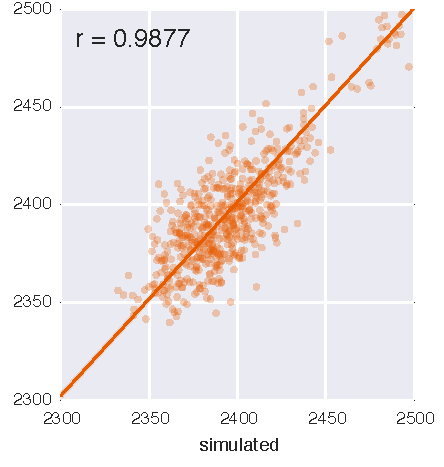
\includegraphics[width=\textwidth]{fig/corr_a.pdf}
                \label{fig:corr_a}
        \end{subfigure}%
        \begin{subfigure}[b]{0.4\textwidth}
                \caption{Optimisation statique/dynamique}
                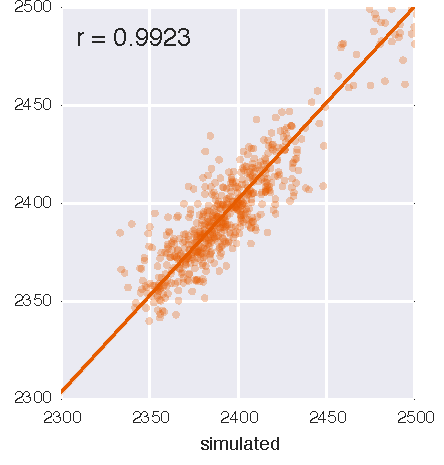
\includegraphics[width=\textwidth]{fig/corr_b.pdf}
                \label{fig:corr_b}
        \end{subfigure}
        \caption{Corrélation de la valeur de densité entre le modèle de
référence et a) 1 réalisation stochastique initiale; b) le modèle obtenu après
optimisation statique/dynamique.}
        \label{fig:corr_rho}
\end{figure}
La corrélation avec le modèle de référence est déjà très bonne après la première
étape du flux de travail (r = \num{0.9877}). Après l'optimisation statique et
dynamique, la corrélation est légèrement améliorée (r = \num{0.9923}). Les
corrélations pour $V_p$, $V_s$ et $\phi$ montrent les mêmes résultats et sont
montrées à la \cref{fig:correlation} de l'article II à la
\cpageref{fig:correlation}.\\
La \cref{fig:qqplot_2} montre le diagramme Quantile-Quantile pour la
distribution de la porosité obtenue à la fin du flux de travail avec la
distribution de la porosité du modèle de référence. Cet outil nous permet de
comparer deux distributions que l'on estime semblables. Dans le cas spécifique,
le diagramme montre un bon alignement avec la première bissectrice, qui indique
la présence d'une identité de loi entre les deux distributions
\citep{Dagnelie2011}.
\begin{figure}[!ht]
\centering
\includegraphics[width=0.4\textwidth]{fig/qqplot_2.pdf}
\caption{Graphique QQ des valeurs de porosité entre le modèle de référence et le
modèle après optimisation statique/dynamique.}
\label{fig:qqplot_2}
\end{figure}
Les diagrammes Quantile-Quantile pour $V_p$, $V_s$ et $\phi$ sont montrés à la
\cref{fig:qqplot} de l'article II à la \cpageref{fig:qqplot} et montrent un bon
alignement avec la première bissectrice, donc une identité de loi entre les
distributions des modèles finaux avec les modèles de référence. \\

Récemment, une mesure de similarité qui compare la tendance structurale locale
entre deux images (SSIM) a été développée par \citet{Wang2004}. La valeur SSIM
est comprise entre \numlist{0;1}, où \num{1} indique que les deux images sont
identiques. La \cref{fig:SSIM_2} compare le modèle de référence avec une
réalisation stochastique initiale (\cref{fig:SSIM_a}) et avec le modèle obtenu
après optimisation (\cref{fig:SSIM_b}) pour la vitesse des ondes $S$ et la
porosité.
\begin{figure}[!ht]
        \centering
        \begin{subfigure}[b]{0.35\textwidth}
                \caption{Réalisation stochastique initiale}
                \includegraphics[width=\textwidth]{fig/SSIM_2_a.pdf}
                \label{fig:SSIM_a}
        \end{subfigure}%
        \begin{subfigure}[b]{0.412\textwidth}
                \caption{Optimisation statique/dynamique}
                \includegraphics[width=\textwidth]{fig/SSIM_2_b.pdf}
                \label{fig:SSIM_b}
        \end{subfigure}
        \caption{SSIM index pour les vitesses des ondes $S$ et la porosité entre
le modèle de référence et a) une réalisation stochastique initiale; b) le modèle
obtenu après optimisation statique/dynamique. La valeur dans l'encadré
correspond à la valeur SSIM moyenne.}
        \label{fig:SSIM_2}
\end{figure}
Le modèle de vitesses des ondes $S$ obtenu après optimisation statique et
dynamique a une similarité avec le modèle de référence deux fois plus grande
en comparaison avec une réalisation initiale. Ce constat est aussi valable pour les
modèles de vitesse des ondes $P$ et la densité, présentés dans la
\cref{fig:SSIM} de l'article II à la \cpageref{fig:SSIM}. Il est intéressant de
noter que le long des forages utilisés pour générer les modèles initiaux
(\numlist{250;500;750}, l'index se rapproche à \num{1}. Ceci est vrai autant
pour les modèles optimisés que pour les modèles stochastiques initiaux. En
effet, les modèles initiaux sont générés en utilisant un algorithme de
cosimulation séquentielle gaussienne qui, par construction, a la caractéristique
de reproduire les observations des puits, c'est-à-dire les données de référence.
On
peut également noter une zone avec un index SSIM très élevée autour de
\SI{750}{\metre} de profondeur et qui correspond à la fine couche des argiles de
la Formation Utica. Comme montré dans la \cref{fig:well-log} de l'article II à
la \cref{fig:well-log}, les distributions des paramètres au niveau de la
Formation Utica sont très proches de la valeur centrale, qui se traduit en une
très faible variabilité et donc un degré de similitude élevée entre les
différents modèles. Ce discours n’est pas valable pour les données de porosité
(\cref{fig:SSIM_b}) qui montrent une valeur moyenne de SSIM très élevée déjà
pour les
réalisations stochastiques initiales. On peut expliquer ceci par le faible
écart-type des distributions de porosité.\\

Enfin, la simulation d’écoulement de \ce{CO2} dans le modèle obtenu après une
réalisation stochastique initiale et dans le modèle obtenu après optimisation statique et dynamique 
est effectuée afin de les comparer avec l'écoulement de \ce{CO2} dans le modèle
de référence. La \cref{fig:CO2_dist} montre l'étendue du panache de \ce{CO2}
pour les trois modèles, tandis que la \cref{fig:SSIM_intro} montre l'index de
similarité structurale entre le modèle de référence et une réalisation initiale
(\cref{fig:SSIM_real}) et entre le modèle de référence et le modèle final
(\cref{fig:SSIM_dg}).
\begin{figure}[!ht]
        \centering
        \begin{subfigure}[b]{0.7\textwidth}
                \caption{Réalisation stochastique initiale}
                \includegraphics[width=\textwidth]{fig/SSIM_real.pdf}
                \label{fig:SSIM_real}
        \end{subfigure}%

        \begin{subfigure}[b]{0.7\textwidth}
                \caption{Modèle obtenu après optimisation statique et dynamique}
                \includegraphics[width=\textwidth]{fig/SSIM_dg.pdf}
                \label{fig:SSIM_dg}
        \end{subfigure}
        \caption{Index de similarité structurelle \citep{Wang2004} du panache du
\ce{CO2} pour la simulation d’écoulement entre le modèle de référence et 1) une
réalisation stochastique initiale; 2) le modèle obtenu après optimisation
statique et dynamique.}
        \label{fig:SSIM_intro}.
\end{figure}
Le degré de similarité, bien que très élevé déjà après une réalisation
stochastique initiale (SSIM = \num{0.88}), est amélioré après l'inversion
stochastique (SSIM = \num{0.92}).
\section{Synthèse des résultats}
Cette section présente une synthèse des résultats obtenus, qui sont discutés
plus
en détail dans l'article II.
Les analyses statistiques présentées dans la section précédente montrent que le
flux de travail proposé permet d'obtenir un modèle final qui montre la meilleure
correspondance
sismique avec le modèle de référence. De plus, l'intégration de la simulation
d'écoulement dans le processus d'optimisation permet d'obtenir le modèle qui
présente la distribution du panache de \ce{CO2} la plus fidèle à la réalité. \\
La méthodologie a été appliquée à un cas synthétique où le modèle de référence a
été obtenu par cosimulation séquentielle gaussienne des données de forages
disponibles dans la zone d'étude et les modèles stochastiques initiaux sont
simulés à partir de trois forages hypothétiques du modèle de référence. Ceci
implique que le modèle de référence et les simulations stochastiques initiales
ont un degré de variabilité limitée, comme il est confirmé par leur corrélation
élevé.\\
Une étape importante pour vérifier l’efficacité de cette méthodologie est donc
l'application à un cas réel qui pourrait confirmer que l'approche proposée
améliore de façon significative l'estimation des paramètres élastiques du
réservoir.
